
%(BEGIN_QUESTION)
% Copyright 2007, Tony R. Kuphaldt, released under the Creative Commons Attribution License (v 1.0)
% This means you may do almost anything with this work of mine, so long as you give me proper credit

Examine this P\&ID:
 
$$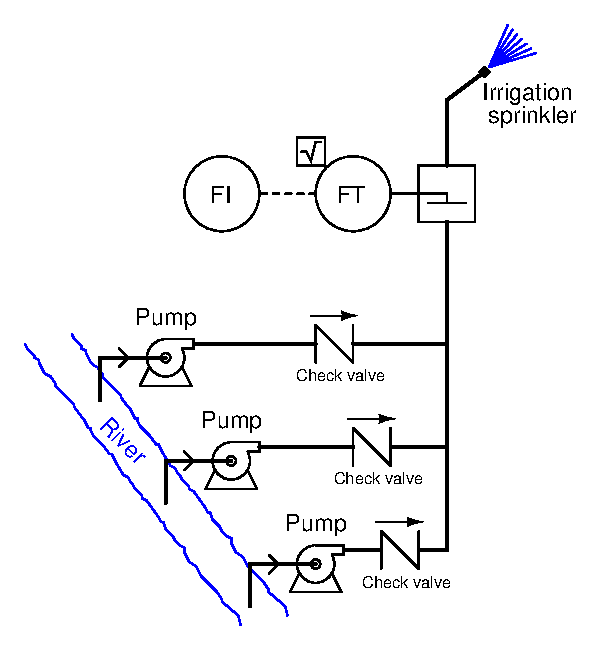
\includegraphics[width=15.5cm]{i01661x01.eps}$$

Three water pumps draw water from a river and deliver it to an irrigation sprinkler.  What will happen to the water flow rate over time if one of the pumps is turned off (the other two pumps left running)?

\vskip 10pt

Would you characterize this process as inherently {\it self-regulating} or inherently {\it integrating}?

\underbar{file i01661}
%(END_QUESTION)





%(BEGIN_ANSWER)

The water flow rate will very quickly decrease, settling at a new (lower) amount of flow.  This makes it a {\it self-regulating} process.

%(END_ANSWER)





%(BEGIN_NOTES)



%INDEX% Control, process characteristics: self-regulating versus integrating

%(END_NOTES)


